\RequirePackage{fix-tudscrfonts} 
\documentclass[ddcfooter, noheader, nototalpages, nosectionnum, svgnames]{tudbeamer}

%Sprache
\usepackage[utf8]{inputenc}
\usepackage[T1]{fontenc}
\usepackage[english]{babel}

%Diagramme + Grafiken
\usepackage{tabularx}
\usepackage{tikz}
\usetikzlibrary{automata, arrows, positioning, matrix, calc, arrows}
\usepackage{subfig}

%Mathesymbole
\usepackage{amssymb}
\usepackage{amsthm}
\usepackage{amsmath}
\usepackage{stmaryrd}

%Operatoren
\DeclareMathOperator*{\argmax}{argmax}
\DeclareMathOperator*{\argmin}{argmin}

%Algorithmus
\usepackage{algorithm}
\usepackage{algorithmicx}
\usepackage{algpseudocode}

%Literatur
\usepackage[backend=biber, style=alphabetic]{biblatex}
\usepackage{csquotes}
\bibliography{../bib/literatur}

%title page
\title{Learning Pruning Policies for Linear Context-free Rewriting Systems}
\subtitle{INF-PM-FPG}
\author{Andy Püschel}
\date{\today}
\einrichtung{Faculty of Computer Science}
\institut{Theoretical Computer Science}
\professur{Chair of Foundations of Programming}

\begin{document}

\setbeamercovered{invisible}
\maketitle

\begin{frame}
	\frametitle{Motivation}
	Example:
	\begin{itemize}
		\item Weighted Deductive Parsing for LCFRS
		\item Sentence
			$w =$ Nun werden sie umworben .
		\item Parser computes the highest scoring derivation $\hat{d}$
	\end{itemize}
\end{frame}

\begin{frame}
	\frametitle{Linear Context-free Rewriting System}
	\begin{definition}
		A \emph{linear context-free rewriting system} is a tuple
		$G =(N, \Sigma, \Xi, P, S)$ where
		\begin{itemize}
			\item $N$ is a finite nonempty $\mathbb{N}$-sorted set (nonterminal symbols),
			\item $\Sigma$ is a finite set (terminal symbols)
				(with $\forall l \in \mathbb{N}: \Sigma \cap N_l = \emptyset$),
			\item $\Xi$ is a finite nontempty set (variable symbols)
				(with $\Xi \cap \Sigma = \emptyset$ and
				$\forall l \in \mathbb{N}: \Xi \cap N_l = \emptyset$),
			\item $P$ is a \emph{set of production rules}
				of the form $\rho = \phi \to \psi$ where
				\begin{itemize}
					\item $\phi = A(\alpha_1, \ldots, \alpha_l)$
						(called left-hand side of $\rho$)\\
						where $l \in \mathbb{N}$, $A \in N_l$,
						$\alpha_1, \ldots, \alpha_l \in (\Sigma \cup \Xi)^*$ and
					\item $\psi = B_1(X^{(1)}_1, \ldots, X^{(1)}_{l_1})
						\ldots B_m(X^{(m)}_1, \ldots, X^{(m)}_{l_m})$
						(called right-hand side of $\rho$)\\
						where $m \in \mathbb{N}$,
						$B_1 \in N_{l_1}, \ldots, B_m \in N_{l_m}$,
						$X^{(i)}_{j} \in \Xi$ for $1 \leq i \leq m, 1 \leq j \leq l_i$
				\end{itemize}
				and for every $X \in \Xi$ occurring in $\rho$ we require that $X$ occurs
				exactly once in the left-hand side of $\rho$ and
				exactly once in the right-hand side of $\rho$, and
			\item $S \in N_1$ (initial nonterminal symbol).
		\end{itemize}
	\end{definition}
\end{frame}

\begin{frame}
	\frametitle{Example PLCFRS}
	PLCFRS $(G, p)$ and $G = (N, \Sigma, \Xi, P, S)$ where
	\begin{itemize}
		\item $N = \{VROOT, S, VP, ADV, VAFIN, VAINF, VVINF, PPER, VVPP, \$, \ldots\}$,
		\item $\Sigma = \{Nun, werden, sie, umworben, ., \ldots\}$ and
		\item $P = \{ \ldots, $
	\begin{align*}
	\only<1>{
		ADV(Nun) \to \varepsilon & \# 1,
		& VAFIN(werden) \to \varepsilon & \# 0,5,\\
		VAINF(werden) \to \varepsilon & \# 0,25,
		& VVINF(werden) \to \varepsilon & \# 0,25,\\
		PPER(sie) \to \varepsilon & \# 1,
		& VVPP(umworben) \to \varepsilon & \# 1,\\
		\$(.) \to \varepsilon & \# 1,}
	\only<2>{
		VP(X_1^{(1)}, X_1^{(2)}) \to ADV(X_1^{(1)}) VVP(X_1^{(2)}) & \# 0,5,\\
		S(X_1^{(1)} X_1^{(2)} X_1^{(3)})
			\to VAFIN(X_1^{(1)}) PPER(X_1^{(2)}) VVPP(X_1^{(3)}) & \# 0,25,\\
		S(X_1^{(1)} X_1^{(2)}, X_2^{(1)})
			\to VP(X_1^{(1)}, X_2^{(1)}) VAINF(X_1^{(2)}) & \# 0,25,\\
		S(X_1^{(1)} X_1^{(2)} X_1^{(3)} X_2^{(1)})
			\to VP(X_1^{(1)}, X_2^{(1)}) VAFIN(X_1^{(2)}) PPER(X_1^{(3)}) & \# 0,5,\\
		S(X_1^{(1)} X_2^{(1)} X_1^{(2)} X_3^{(1)})
			\to S(X_1^{(1)} X_2^{(1)}, X_3^{(1)}) PPER(X_1^{(2)}) & \# 0,25,\\
		VROOT(X_1^{(1)} X_2^{(1)} X_3^{(1)} X_4^{(1)} X_1^{(2)})
			\to S(X_1^{(1)} X_2^{(1)} X_3^{(1)} X_4^{(1)}) \$(X_1^{(2)}) & \# 1}
	\end{align*}
	$, \ldots\}$
	\end{itemize}
\end{frame}

\begin{frame}
	\frametitle{\textproc{Parse} - Weighted Deductive Parsing:\\ Nun werden sie umworben .}
	\begin{figure}[t]
		\begin{overlayarea}{\textwidth}{\textheight}
			\centering
			\only<1>{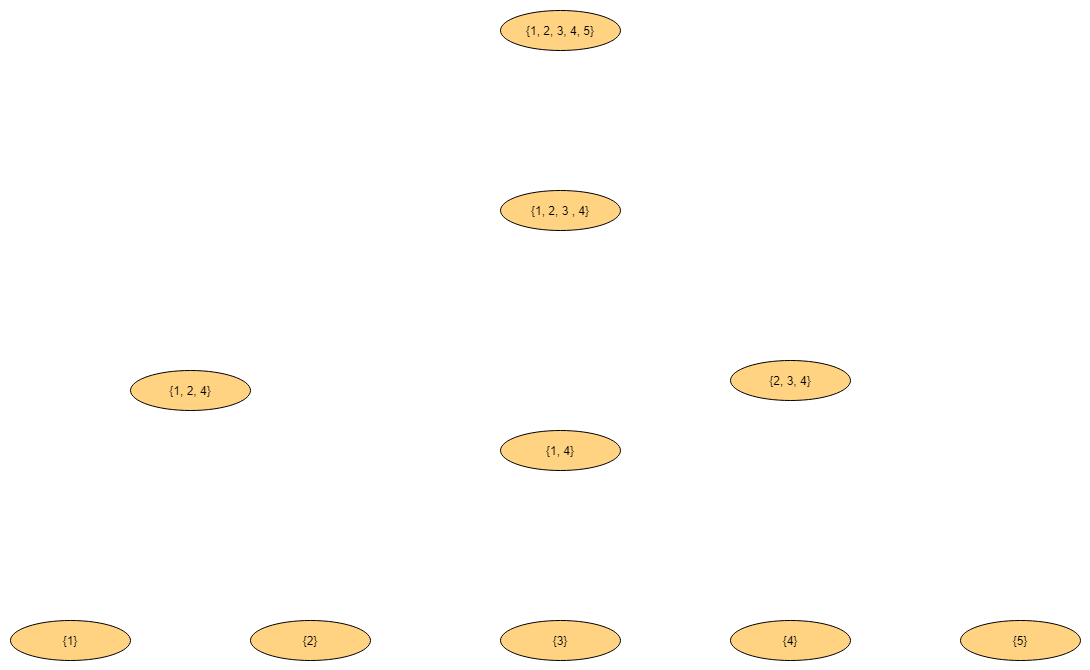
\includegraphics[width=0.8\textwidth]{../img/parse_01.png}\\
				Initialize vertives}
			\only<2>{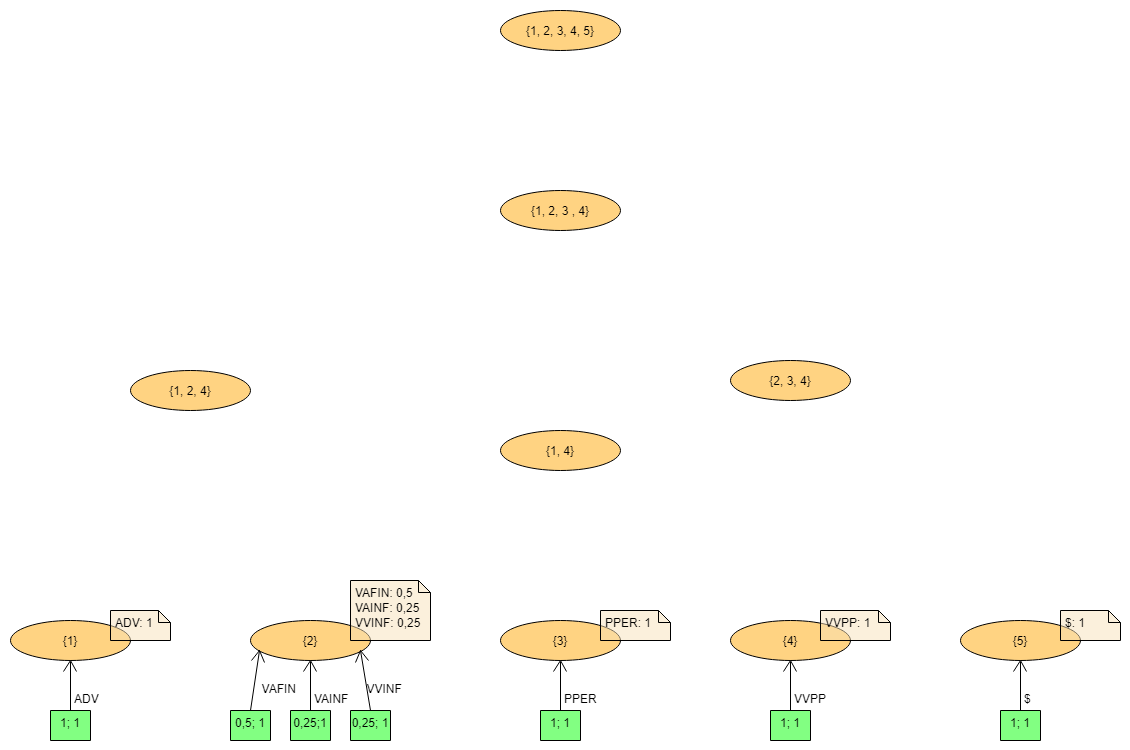
\includegraphics[width=0.8\textwidth]{../img/parse_02.png}\\
				hyperedges for $ADV(Nun) \to \varepsilon \# 1, \ldots$}
			\only<3>{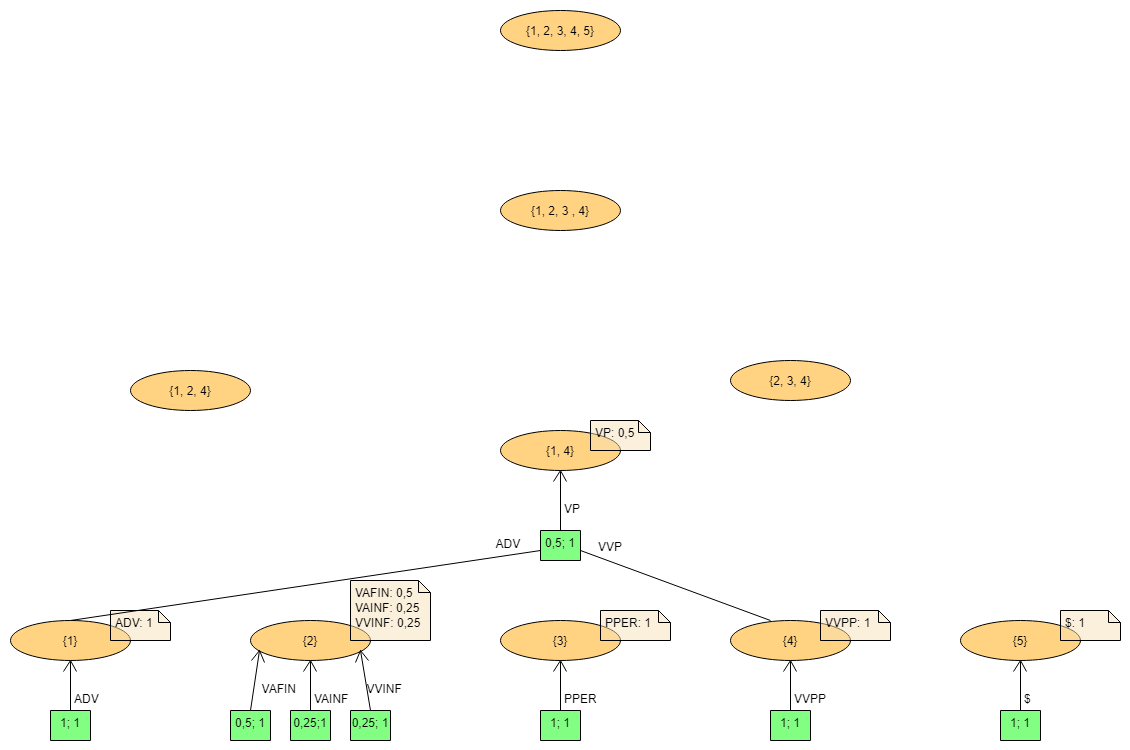
\includegraphics[width=0.8\textwidth]{../img/parse_03.png}\\
				hyperedge for $VP(X_1^{(1)}, X_1^{(2)}) 
				\to ADV(X_1^{(1)}) VVP(X_1^{(2)}) \# 0,5$}
			\only<4>{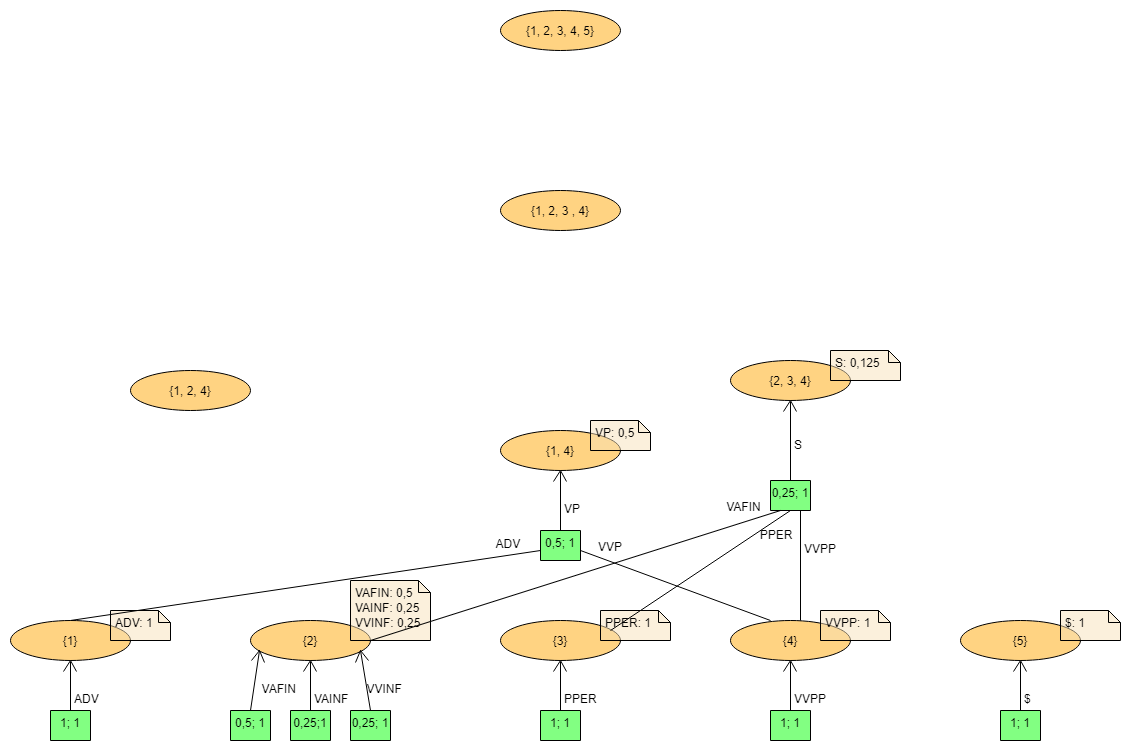
\includegraphics[width=0.8\textwidth]{../img/parse_04.png}\\
				hyperedge for $S(X_1^{(1)} X_1^{(2)} X_1^{(3)})
				\to VAFIN(X_1^{(1)}) PPER(X_1^{(2)}) VVPP(X_1^{(3)}) \# 0,25$}
			\only<5>{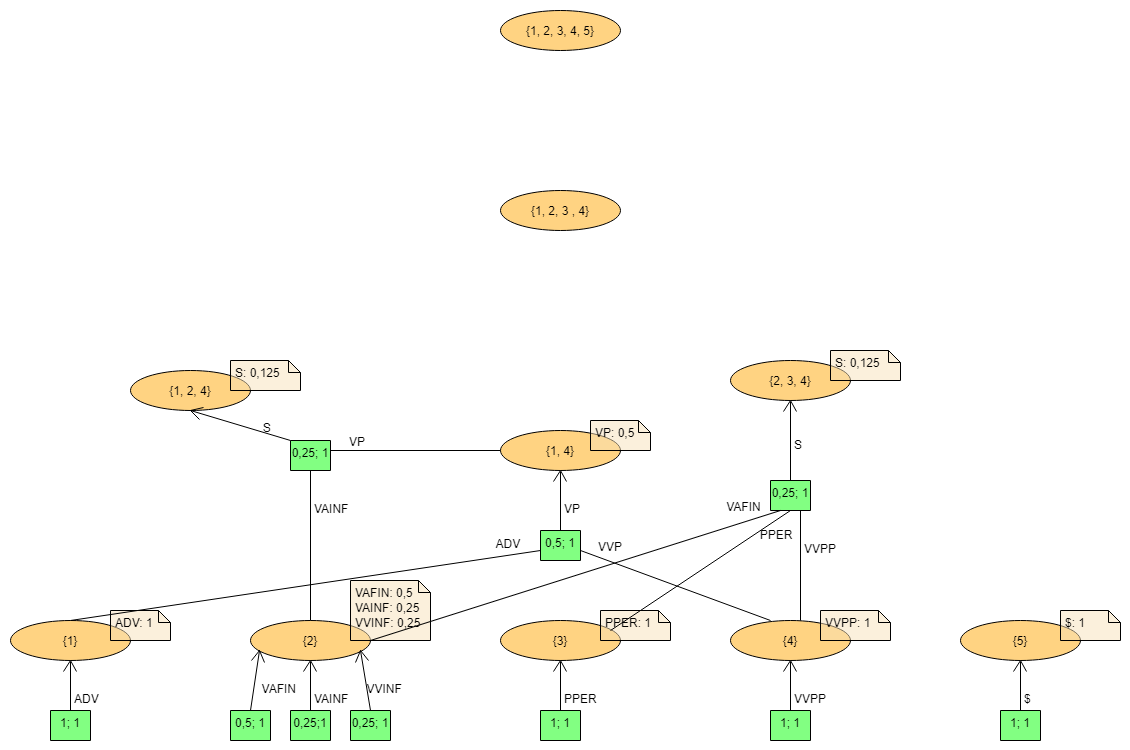
\includegraphics[width=0.8\textwidth]{../img/parse_05.png}\\
				hyperedge for $S(X_1^{(1)} X_1^{(2)}, X_2^{(1)})
				\to VP(X_1^{(1)}, X_2^{(1)}) VAINF(X_1^{(2)}) \# 0,25$}
			\only<6>{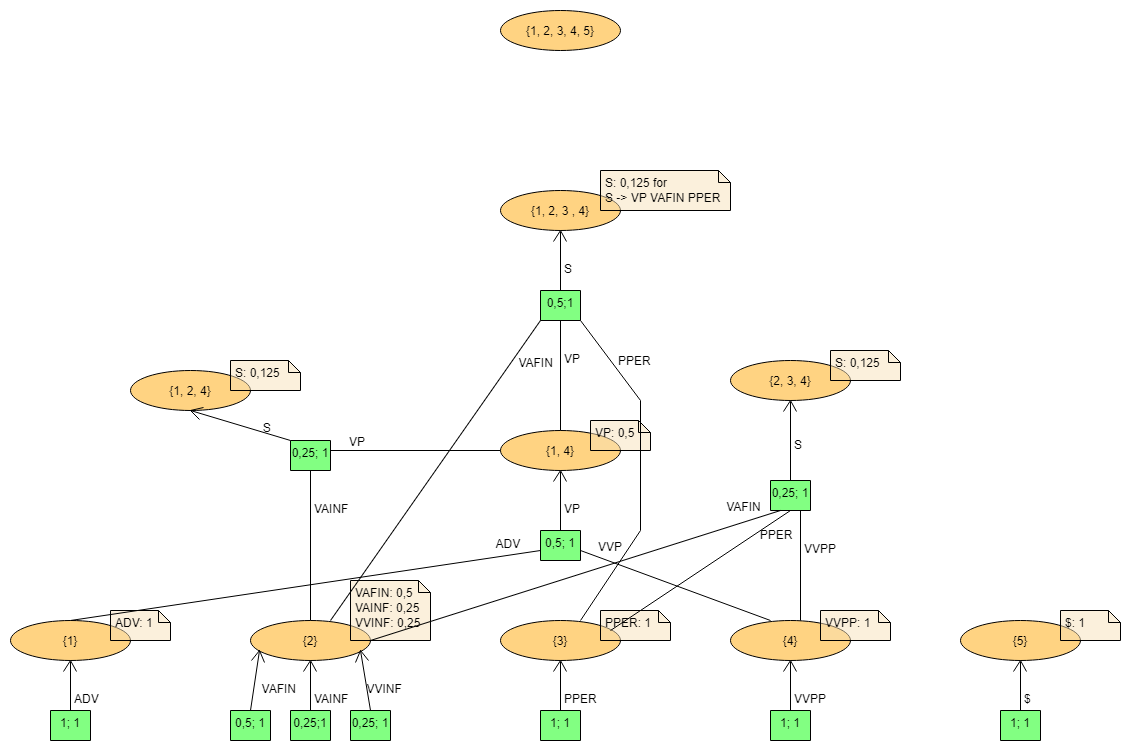
\includegraphics[width=0.8\textwidth]{../img/parse_06.png}\\
				hyperedge for $S(X_1^{(1)} X_1^{(2)} X_1^{(3)} X_2^{(1)})
				\to VP(X_1^{(1)}, X_2^{(1)}) VAFIN(X_1^{(2)}) PPER(X_1^{(3)}) \# 0,5$}
			\only<7>{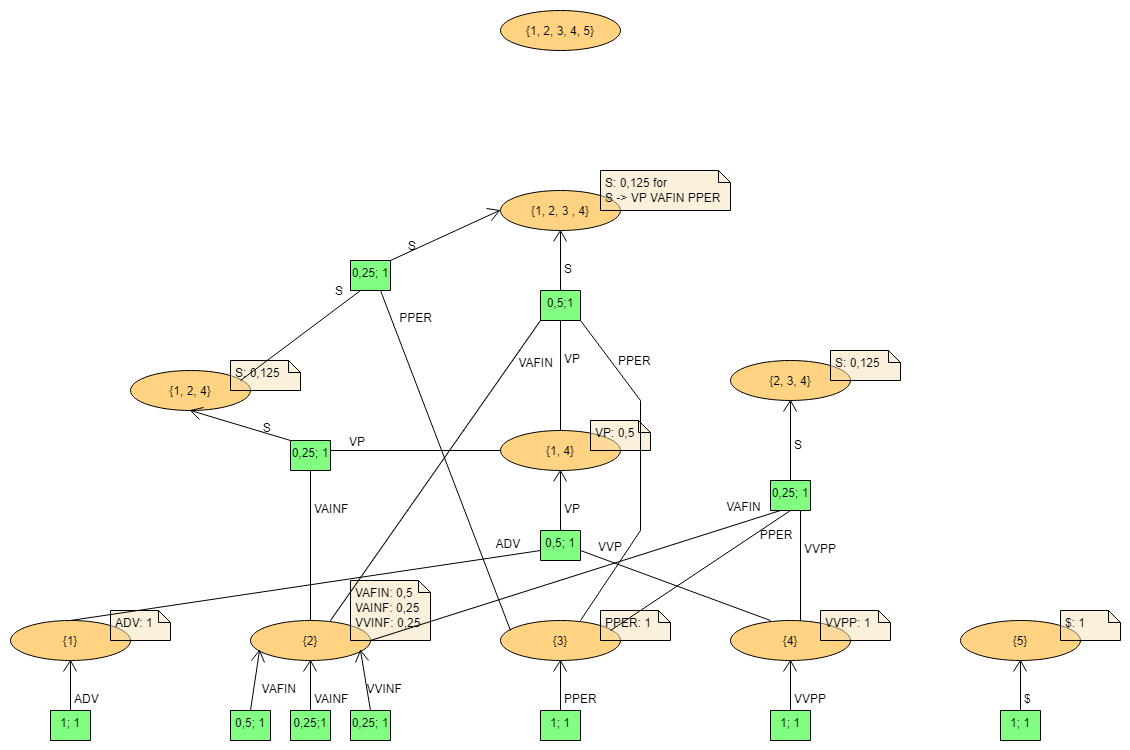
\includegraphics[width=0.8\textwidth]{../img/parse_07.png}\\
				hyperedge for $S(X_1^{(1)} X_2^{(1)} X_1^{(2)} X_3^{(1)})
				\to S(X_1^{(1)} X_2^{(1)}, X_3^{(1)}) PPER(X_1^{(2)}) \# 0,25$}
			\only<8>{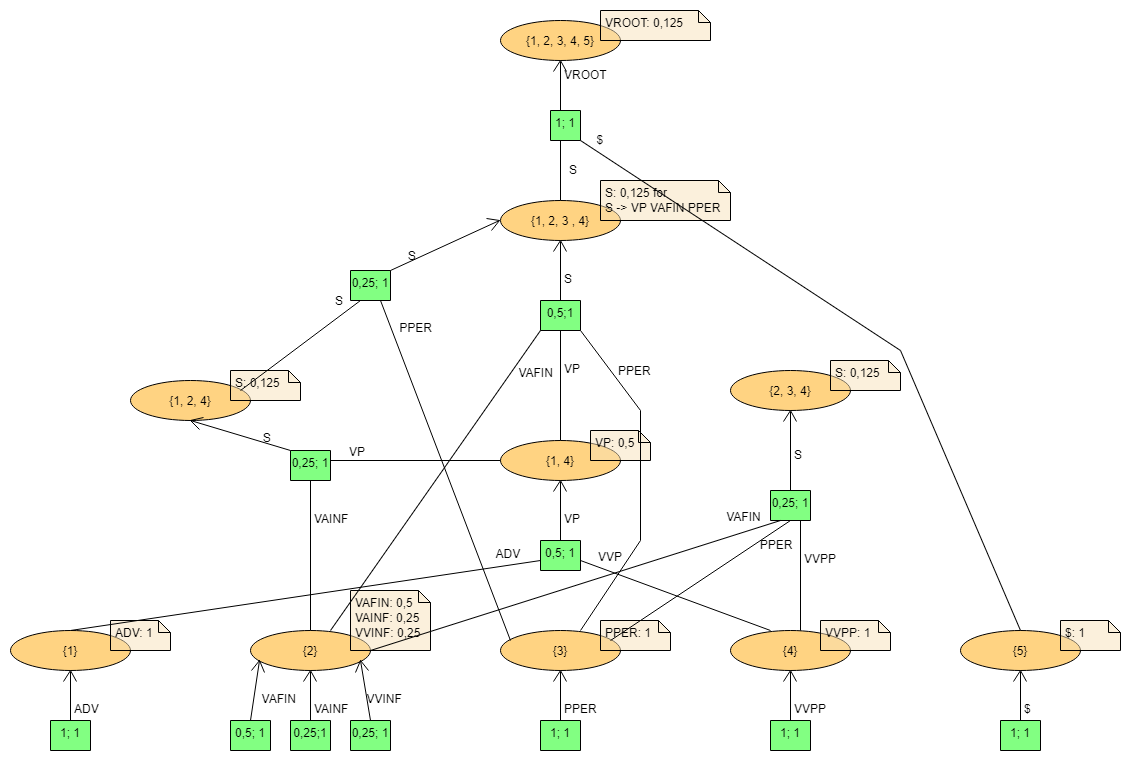
\includegraphics[width=0.8\textwidth]{../img/parse_08.png}\\
				hyperedge for $VROOT(X_1^{(1)} X_2^{(1)} X_3^{(1)} X_4^{(1)} X_1^{(2)})
				\to S(X_1^{(1)} X_2^{(1)} X_3^{(1)} X_4^{(1)}) \$(X_1^{(2)}) \# 1$}
			\only<9>{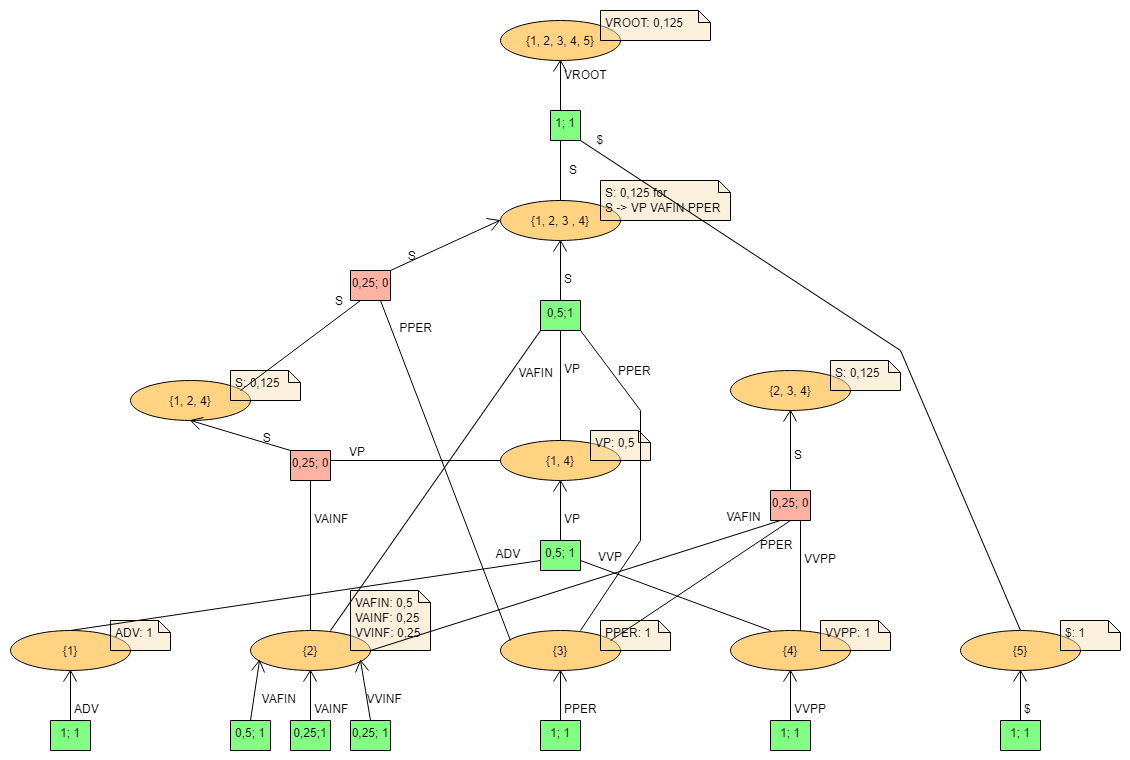
\includegraphics[width=0.8\textwidth]{../img/parse_09.png}\\
				Undesired hyperedges}
			\only<10>{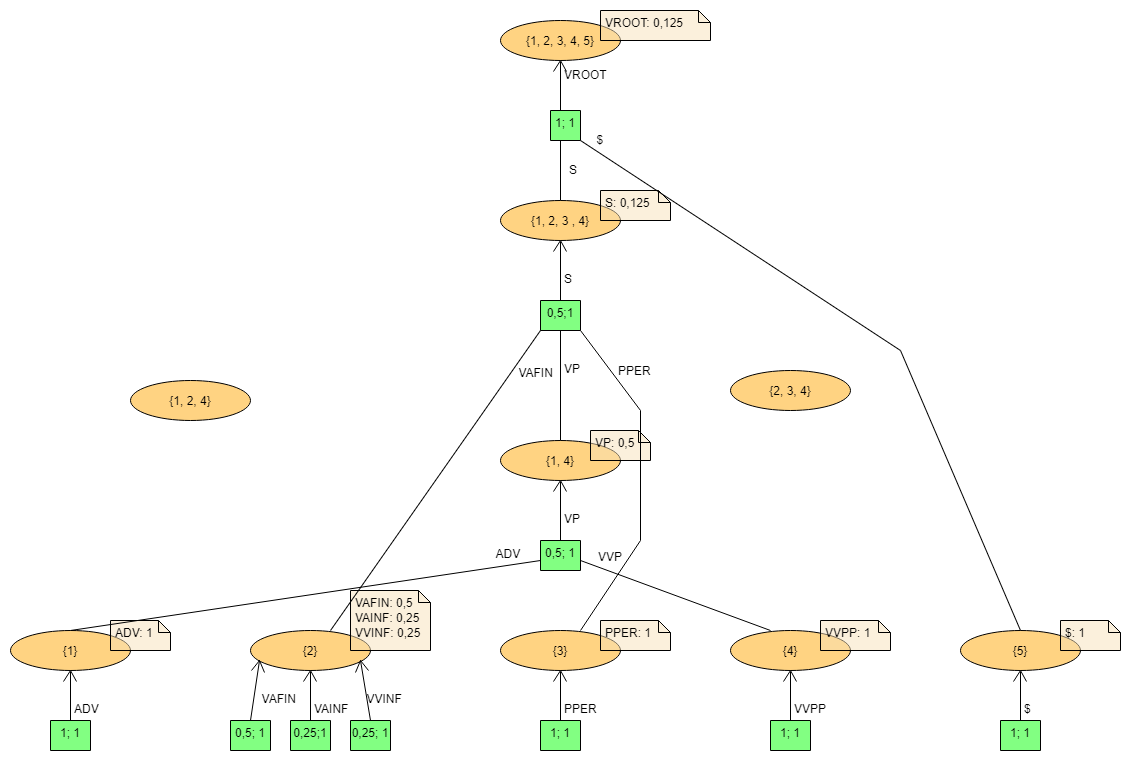
\includegraphics[width=0.8\textwidth]{../img/parse_10.png}\\
				Prune}
		\end{overlayarea}
	\end{figure}
\end{frame}

\begin{frame}
	\frametitle{Motivation}
	\begin{itemize}[<+->]
		\item How to reduce the parse time for a sentence?
		\item What is a good pruning method?
		\item How to train such a pruning method?
	\end{itemize}
\end{frame}

\begin{frame}
	\frametitle{Overview}
	\begin{itemize}
		\item \textcolor{Grey}{Motivation}
		\item Preliminaries
		\item \textproc{Lols}
		\item \textcolor{Grey}{Change Propagation}
		\item \textcolor{Grey}{Dynamic Programming}
		\item \textcolor{Grey}{Results}
	\end{itemize}
\end{frame}

\begin{frame}
	\frametitle{Preliminaries}
	\begin{align*}
		H = (V, E) \in \mathcal{H}_{(G, p)}(w) &:
			\text{derivation graph from \textproc{Parse}}\\
		c \subset \Sigma^* \times T_N(\Sigma)&: X \times Y-\text{corpus}\\
		s &: \text{state of the derivation graph}\\
		a \in \{\textcolor{Green}{keep}, \textcolor{Red}{prune}\} &: \text{action}\\
		\tau = s_0a_0s_1a_1\ldots s_T &: \text{trajectory}
	\end{align*}
\end{frame}

\begin{frame}
	\frametitle{Preliminaries}
	\begin{align*}
		\text{pruning policy } \pi &: \text{inputs a hyperedge and a sub sentence } w'\\
			& \text{outputs a pruning decision }
				a \in \{\textcolor{Green}{keep}, \textcolor{Red}{prune}\}
	\end{align*}
	How to evaluate $\pi$?
	\visible<2>
	{
		\begin{align*}
			\text{reward function } r &:
				\mathcal{H}_{(G, p)}(w) \times T_N(\Sigma) \to \mathbb{R}\\
			\text{schematically } r &= accuracy - \lambda \cdot runtime\\
			\text{where } accuracy &: T_N(\Sigma) \times T_N(\Sigma) \to \mathbb{R}\\
			\text{and } runtime &: \mathcal{H}_{(G, p)}(w) \to \mathbb{R}\\
			\lambda \in \mathbb{R} &: \text{trade-off factor}\\
			\text{empirical value of } \pi &: \mathcal{R}(\pi) =
				\frac{1}{|c|}\sum_{(w, \xi) \in c}
				r(\textproc{Parse}(G, w, \pi), \xi) \cdot c(w, \xi)
		\end{align*}
	}
\end{frame}

\begin{frame}
	\frametitle{Preliminaries}
	trajectory: $s_0a_0s_1a_1 \ldots s_T$ \visible<2->{, (intervention at state $s_1$)}
	\begin{figure}
		\centering
		\scalebox{0.9}{\begin{tikzpicture}[->,>=stealth',shorten >=1pt, auto, thick, every text node part/.style={align=center}]
	\only<1-2>
	{
		\node[inner sep=0pt, label=above:$s_1$] (i) {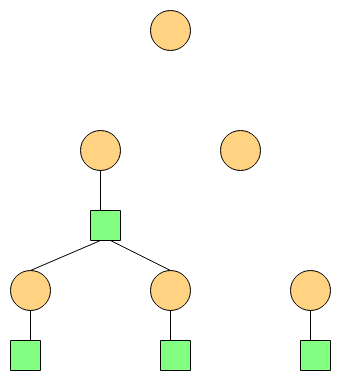
\includegraphics[scale=0.2]{../img/trajectory_i.png}};
		\node[inner sep=0pt, right=of i, label=above:$s_2$] (k1) {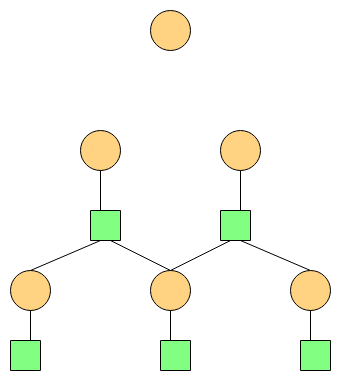
\includegraphics[scale=0.2]{../img/trajectory_k1.png}};
		\node[draw=none, right=of k1](E1){$\ldots$};
		\node[inner sep=0pt, right=of E1, label=above:$s_T$] (k2) {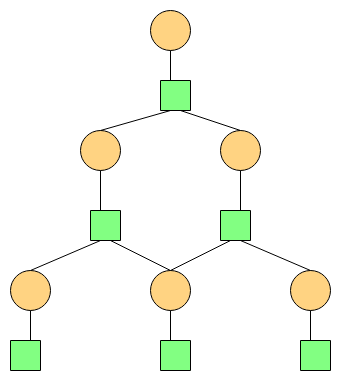
\includegraphics[scale=0.2]{../img/trajectory_k2.png}};
    \node[draw=none, right=0pt of k2](R1){$\vec{r}_1[a_1]$};
		
		\path[->]
		  (i) edge node[above]{$a_1$} (k1)
  		(k1) edge node[above]{$a_2$} (E1)
  		(E1) edge node[above]{$a_{T-1}$} (k2);
	}
	\visible<2>
	{
		\node[inner sep=0pt, below=of k1, label=above:$s_2'$] (p1) {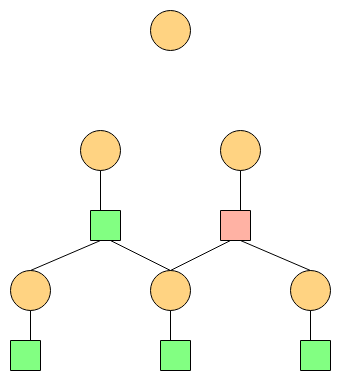
\includegraphics[scale=0.2]{../img/trajectory_p1.png}};
		\node[draw=none, right=of p1](E2){$\ldots$};
		\node[inner sep=0pt, right=of E2, label=above:$s_T'$] (p2) {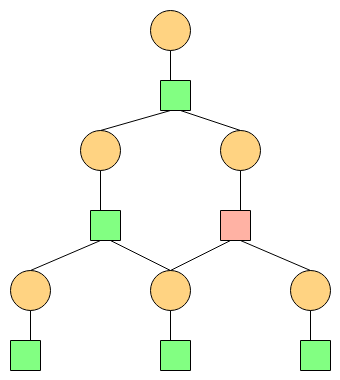
\includegraphics[scale=0.2]{../img/trajectory_p2.png}};
    \node[draw=none, right=0pt of p2](R2){$\vec{r}_1[a_1']$};
		
		\path[->]
  		(p1) edge node[above]{$a_2'$} (E2)
  		(E2) edge node[above]{$a_{T-1}'$} (p2)
  		(i) edge[bend right] node[above]{$a_1'$}(p1); 
	}
\end{tikzpicture} 
}
	\end{figure}
\end{frame}

\begin{frame}
	\frametitle{LOLS}
	\framesubtitle{Locally Optimal Learning to Search}
	\begin{center}
		\scalebox{0.55}
		{
			\begin{minipage}{1.5\linewidth}
				\renewcommand{\algorithmicrequire}{\textbf{Input:}}
\renewcommand{\algorithmicensure}{\textbf{Output:}}
\renewcommand{\Comment}[2][.5\linewidth]{%
	\leavevmode\hfill\makebox[#1][l]{$\triangleright$~#2}}

\begin{algorithm}[H]
	\caption{Locally Optimal Learning to Search algorithm
		by \cite{vieira17} and \cite{chang15}}
	\label{alg:lols}
	\begin{algorithmic}[1]
		\Require PLCFRS $(G, p)$ with $G = (N, \Sigma, \Xi, P, S)$,
		\Statex $X\times Y$-corpus $c$ such that $X \subset \Sigma^*$
			and $Y \subset T_N(\Sigma)$
		\Ensure pruning policy $\pi$
		\Statex
		\Function{Lols}{$(G, p), c$}
			\State $\pi_1 := $ \textcolor{Purple}{\textproc{InitializePolicy}}($\ldots$)
			\For{$i := 1$ to $n$} \Comment{$n$ : number of iterations}
				\State $Q_i := \emptyset$ \Comment{$Q_i$ : set of state-reward tuples}
				\For{$(w, \xi) \in c$} \Comment{$w$ : sentence}
					\State $\tau :=$
						\textcolor{Purple}{\textproc{Roll-In}}($(G, p), w, \pi _i, \xi$)
					\Comment{$\tau = s_0a_0s_1a_1 \ldots s_T$ : trajectory}
					\For{$t := 0$ to $|\tau | - 1$}
						\For{$\bar{a}_t \in 
							\{\textcolor{Green}{keep}, \textcolor{Tomato}{prune}\}$}
							\Comment{intervention}
							\State $\vec{r}_t[a'_t] :=$
								\textcolor{Purple}{\textproc{Roll-Out}}
									($\pi_i, s_t, a'_t, \xi$)
						\EndFor
						\State $Q_i := Q_i \cup \{(s_t, \vec{r}_t)\}$
					\EndFor
				\EndFor
				\State $\pi_{i+1} :=$
					\textcolor{Purple}{\textproc{Train}}($\bigcup^{i}_{k=1} Q_k$)
					\Comment{dataset aggregation}
			\EndFor
			\State \Return $\argmax_{\pi_j:1 \leq j \leq n}\mathcal{R}(\pi_j)$
		\EndFunction
	\end{algorithmic}
\end{algorithm}
			\end{minipage}
		}
	\end{center}
\end{frame}

\begin{frame}
	\frametitle{Overview}
	\begin{itemize}
		\item \textcolor{Grey}{Motivation}
		\item \textcolor{Grey}{Preliminaries}
		\item \textcolor{Grey}{\textproc{Lols}}
		\item Change Propagation
		\item \textcolor{Grey}{Results}
	\end{itemize}
\end{frame}

\begin{frame}
	\frametitle{Change Propagation}
	\begin{figure}
		\begin{overlayarea}{\textwidth}{\textheight}
			\centering
			\only<1>{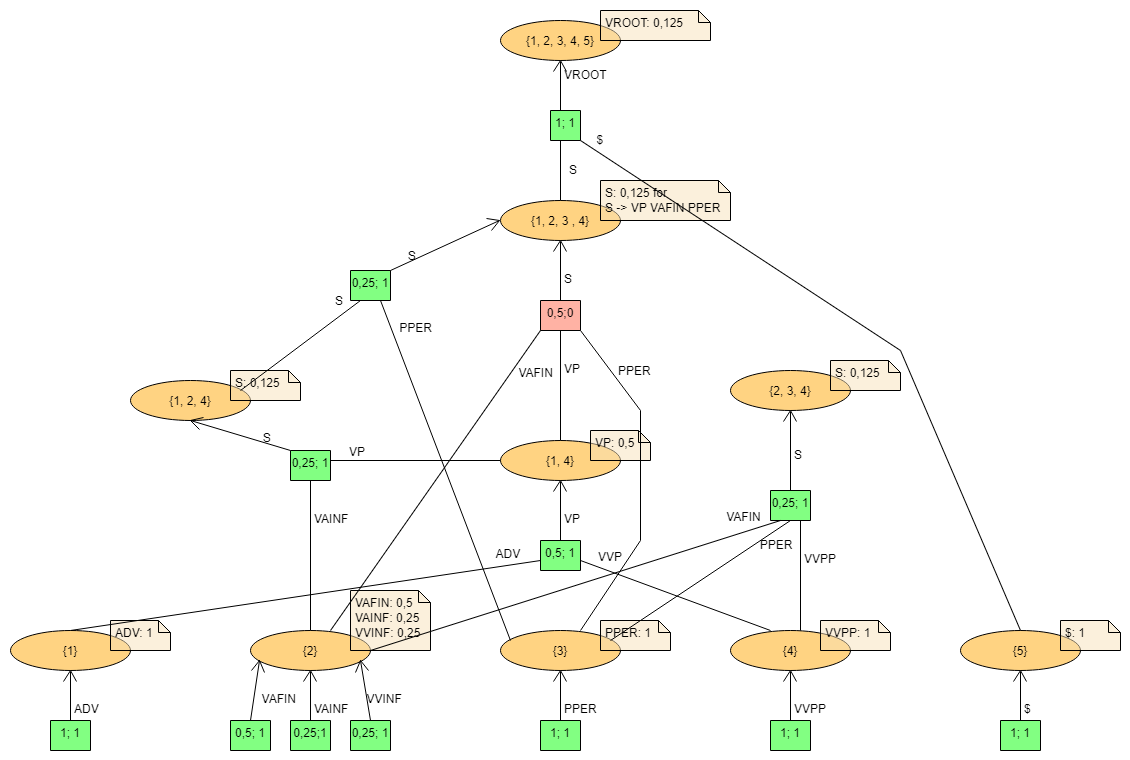
\includegraphics[width=0.8\textwidth]{../img/cp_1.png}\\
				Change pruning bit}
			\only<2>{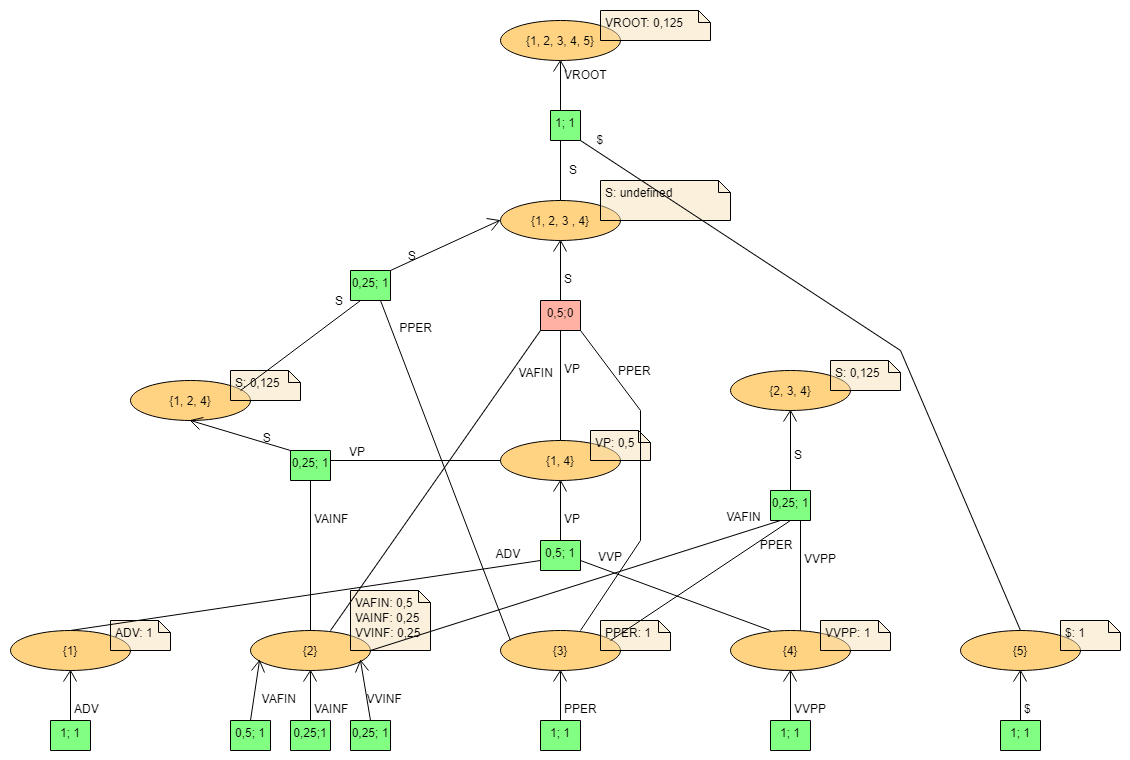
\includegraphics[width=0.8\textwidth]{../img/cp_2.png}\\
				Delete witness for $\{1, 2, 3, 4\}$ and S}
			\only<3>{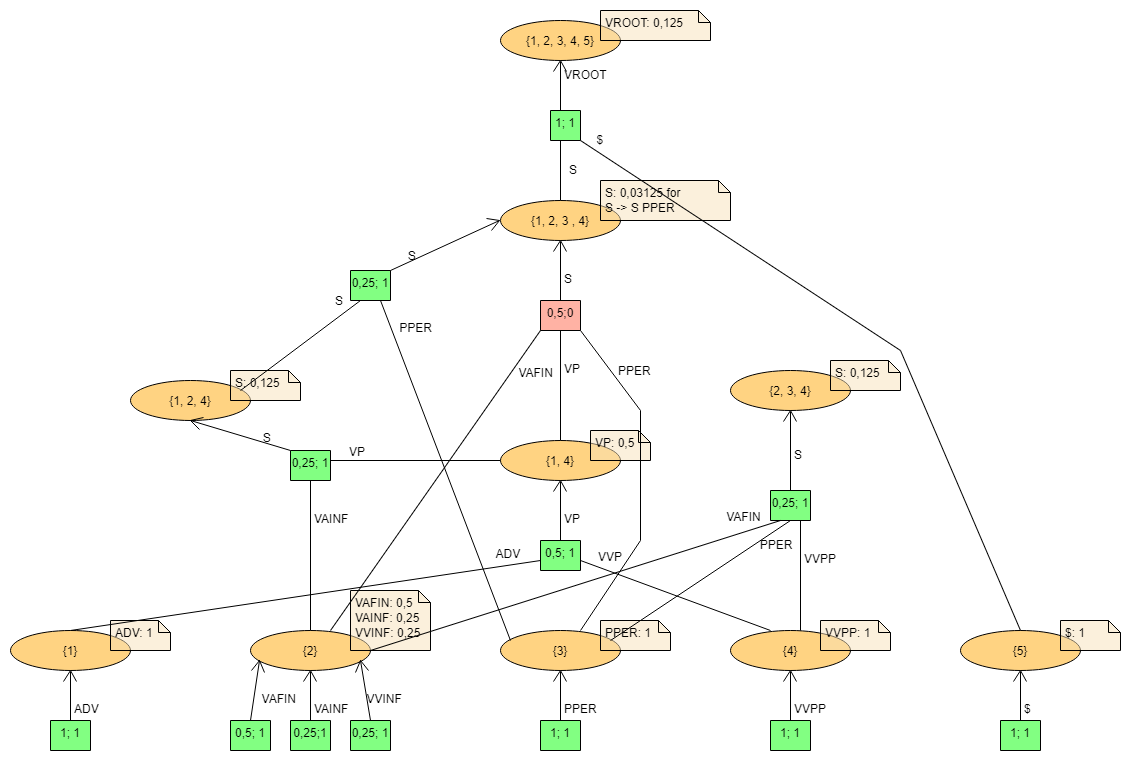
\includegraphics[width=0.8\textwidth]{../img/cp_3.png}\\
				Find new witness for $\{1, 2, 3, 4\}$ and S}
			\only<4>{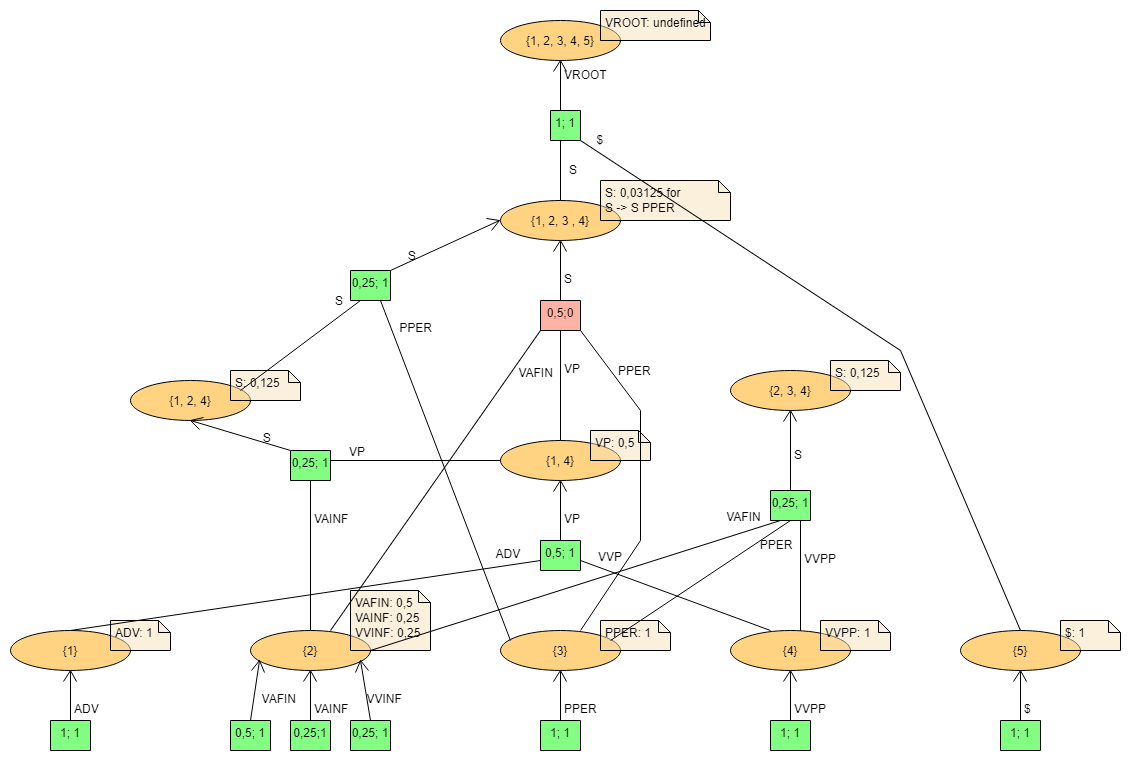
\includegraphics[width=0.8\textwidth]{../img/cp_4.png}\\
				Repeat for affected vertices}
			\only<5>{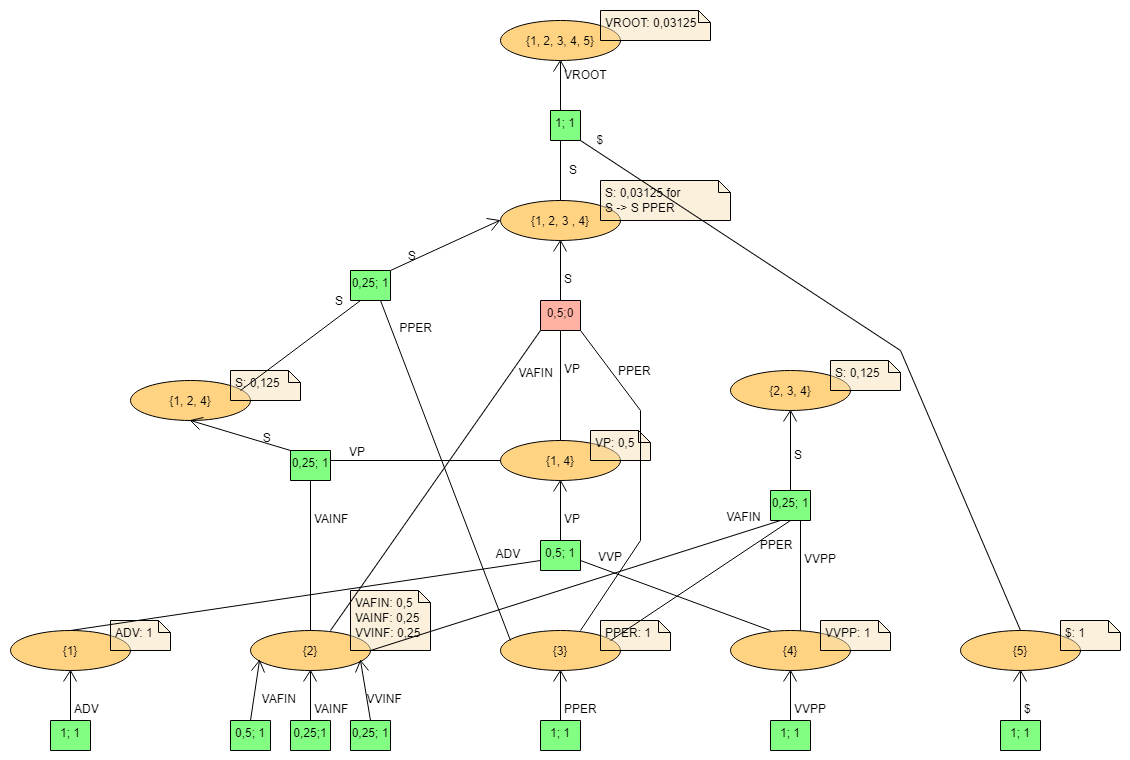
\includegraphics[width=0.8\textwidth]{../img/cp_5.png}\\
				Done}
		\end{overlayarea}
	\end{figure}
\end{frame}

\begin{frame}
	\frametitle{Overview}
	\begin{itemize}
		\item \textcolor{Grey}{Motivation}
		\item \textcolor{Grey}{Preliminaries}
		\item \textcolor{Grey}{\textproc{Lols}}
		\item \textcolor{Grey}{Change Propagation}
		\item Results
	\end{itemize}
\end{frame}

\begin{frame}
	\frametitle{Accuracy Measure}
	\begin{overlayarea}{\textwidth}{0.5\textheight}
		\only<1>
		{
			\begin{figure}
				\scalebox{0.6}{\begin{tikzpicture}
	\draw (4,0) -- (0,0) -- (0,7) -- (8,7) -- (8,0) -- (4,0) -- (4,7);
	\draw (4,3) ellipse (3cm and 2cm);
	\node (FN) at (2,6) {$FN$};
	\node (TN) at (6,6) {$TN$};
	\node (TP) at (3,3) {$TP$};
	\node (FP) at (5,3) {$FP$};
	\node (RC) at (2,7.5) {Relevant Elements};
\end{tikzpicture}}
			\end{figure}
		}
		\only<2->
		{
			\begin{columns}
				\column[t]{0.5\textwidth}
				derivation tree by parsing
				\begin{figure}
					\only<2>{\scalebox{0.75}{\begin{tikzpicture}
	%nodes
	\node[name=S, circle, fill=White]{S};
	\node[name=NP, circle, fill=White, below left=of S]{NP};
	\node[name=VP, circle, fill=White, below right=of S]{VP};
	\node[name=NP2, circle, fill=White, below=of VP]{NP};
	\node[name=NP3, circle, fill=White, below left=of NP2]{NP};
	\node[name=PP, circle, fill=White, below right=of NP2]{PP};
	%path
	\path
		(S) edge (NP)
		(S) edge (VP)
		(VP) edge (NP2)
		(NP2) edge (NP3)
		(NP2) edge (PP);
\end{tikzpicture}}}
					\only<3>{\scalebox{0.75}{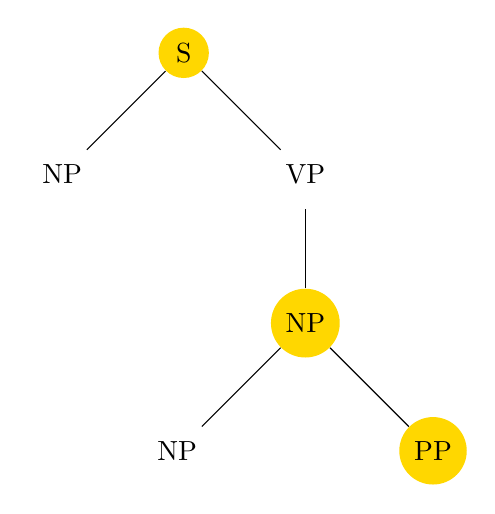
\begin{tikzpicture}
	%nodes
	\node[name=S, circle, fill=Gold]{S};
	\node[name=NP, circle, fill=White, below left=of S]{NP};
	\node[name=VP, circle, fill=White, below right=of S]{VP};
	\node[name=NP2, circle, fill=Gold, below=of VP]{NP};
	\node[name=NP3, circle, fill=White, below left=of NP2]{NP};
	\node[name=PP, circle, fill=Gold, below right=of NP2]{PP};
	%path
	\path
		(S) edge (NP)
		(S) edge (VP)
		(VP) edge (NP2)
		(NP2) edge (NP3)
		(NP2) edge (PP);
\end{tikzpicture}}}
					\only<4->{\scalebox{0.75}{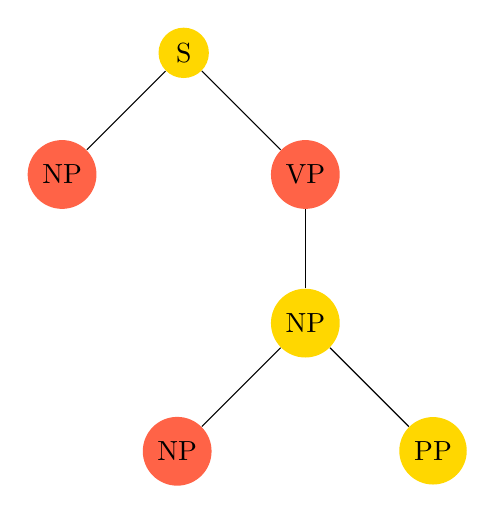
\begin{tikzpicture}
	%nodes
	\node[name=S, circle, fill=Gold]{S};
	\node[name=NP, circle, fill=Tomato, below left=of S]{NP};
	\node[name=VP, circle, fill=Tomato, below right=of S]{VP};
	\node[name=NP2, circle, fill=Gold, below=of VP]{NP};
	\node[name=NP3, circle, fill=Tomato, below left=of NP2]{NP};
	\node[name=PP, circle, fill=Gold, below right=of NP2]{PP};
	%path
	\path
		(S) edge (NP)
		(S) edge (VP)
		(VP) edge (NP2)
		(NP2) edge (NP3)
		(NP2) edge (PP);
\end{tikzpicture}}}
				\end{figure}
				\column[t]{0.5\textwidth}
				derivation tree by gold standard
				\begin{figure}
					\only<2>{\scalebox{0.75}{\begin{tikzpicture}
	%nodes
	\node[name=S, circle, fill=White]{S};
	\node[name=CNP, circle, fill=White, below left=of S]{CNP};
	\node[name=NP, circle, fill=White, below right=of S]{NP};
	\node[name=PP, circle, fill=White, below=of NP]{PP};
	%path
	\path
		(S) edge (CNP)
		(S) edge (NP)
		(NP) edge (PP);
\end{tikzpicture}}}
					\only<3>{\scalebox{0.75}{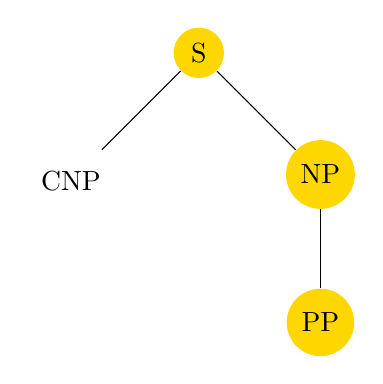
\begin{tikzpicture}
	%nodes
	\node[name=S, circle, fill=Gold]{S};
	\node[name=CNP, circle, fill=White, below left=of S]{CNP};
	\node[name=NP, circle, fill=Gold, below right=of S]{NP};
	\node[name=PP, circle, fill=Gold, below=of NP]{PP};
	%path
	\path
		(S) edge (CNP)
		(S) edge (NP)
		(NP) edge (PP);
\end{tikzpicture}}}
					\only<4->{\scalebox{0.75}{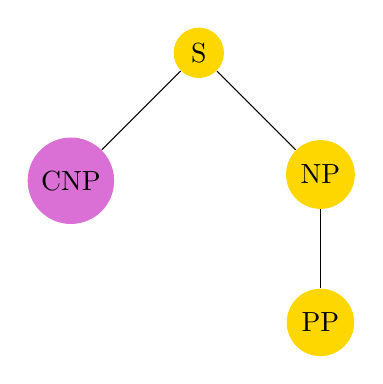
\begin{tikzpicture}
	%nodes
	\node[name=S, circle, fill=Gold]{S};
	\node[name=CNP, circle, fill=Orchid, below left=of S]{CNP};
	\node[name=NP, circle, fill=Gold, below right=of S]{NP};
	\node[name=PP, circle, fill=Gold, below=of NP]{PP};
	%path
	\path
		(S) edge (CNP)
		(S) edge (NP)
		(NP) edge (PP);
\end{tikzpicture}}}
				\end{figure}
			\end{columns}
		}
	\end{overlayarea}
	\begin{align*}
		\text{precision} &= \frac{|TP|}{|TP|+|FP|}
		&\text{recall} &= \frac{|TP|}{|TP|+|FN|}\\
		\mathfrak{p}(\xi) &=
		\frac{\visible<3->{3}}
			{\visible<3->{3}\visible<4->{+ 3}}
		\visible<5->{=0,5}
		&\mathfrak{r}(\xi) &=
		\frac{\visible<3->{3}}
			{\visible<3->{3}\visible<4->{+ 1}}
		\visible<5->{= 0,75}
	\end{align*}
\end{frame}

\begin{frame}
	\frametitle{Setup}
	\begin{align*}
		accuracy(\xi, \zeta) &= 2 \cdot
			\frac{\mathfrak{p}(\xi, \zeta) \cdot \mathfrak{r}(\xi, \zeta)}
			{\mathfrak{p}(\xi, \zeta) + \mathfrak{r}(\xi, \zeta)}
		& \text{ F1-Measure},\\
		runtime(H) &= |E|
		& \text{ for } H = (V, E)\\
		\lambda &\in [0, 1]
	\end{align*}
\end{frame}

\begin{frame}
	\frametitle{Results}
	\begin{figure}
    	\centering
    	\subfloat[accuracy for $\lambda$]{{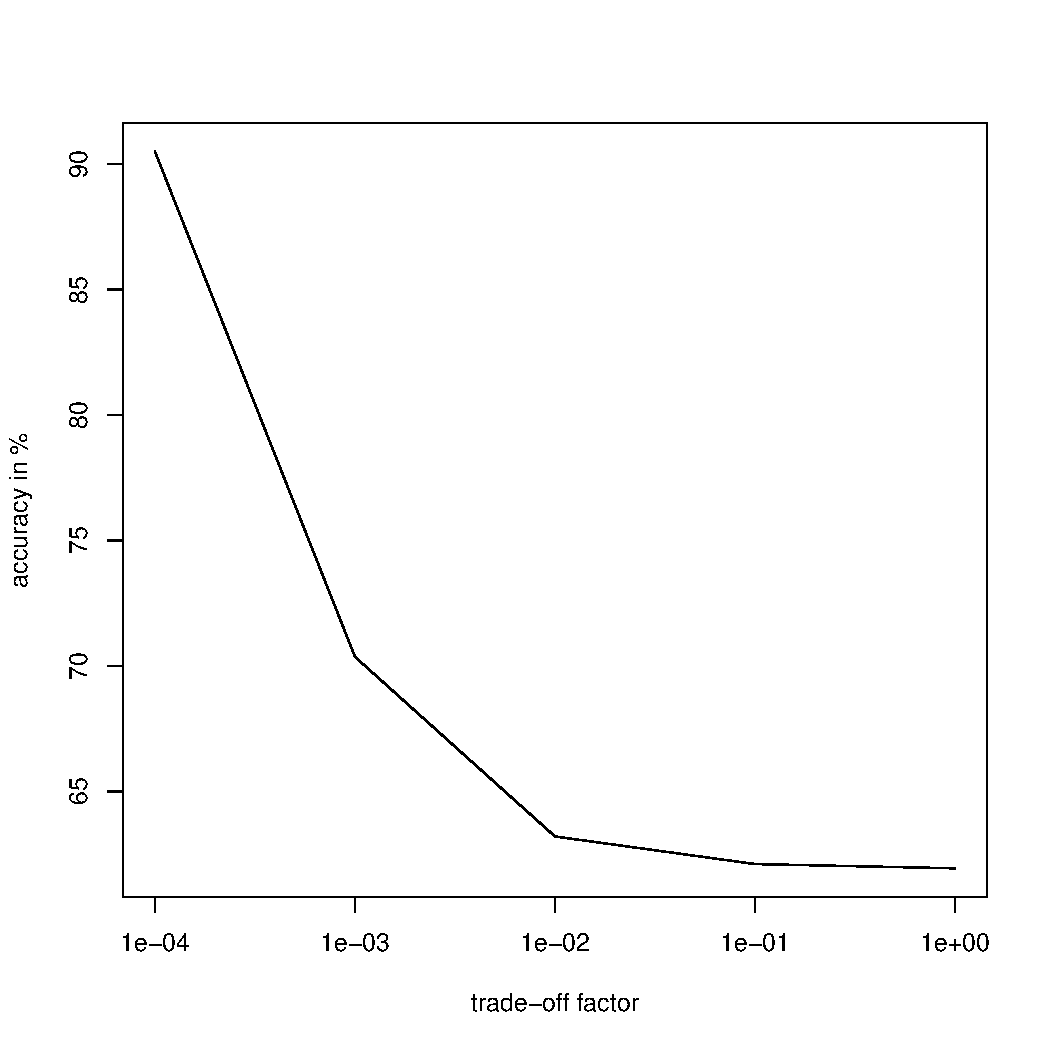
\includegraphics[width=0.45\textwidth]{../dia/accuracy.pdf} }}
    	\qquad
    	\subfloat[runtime for $\lambda$]{{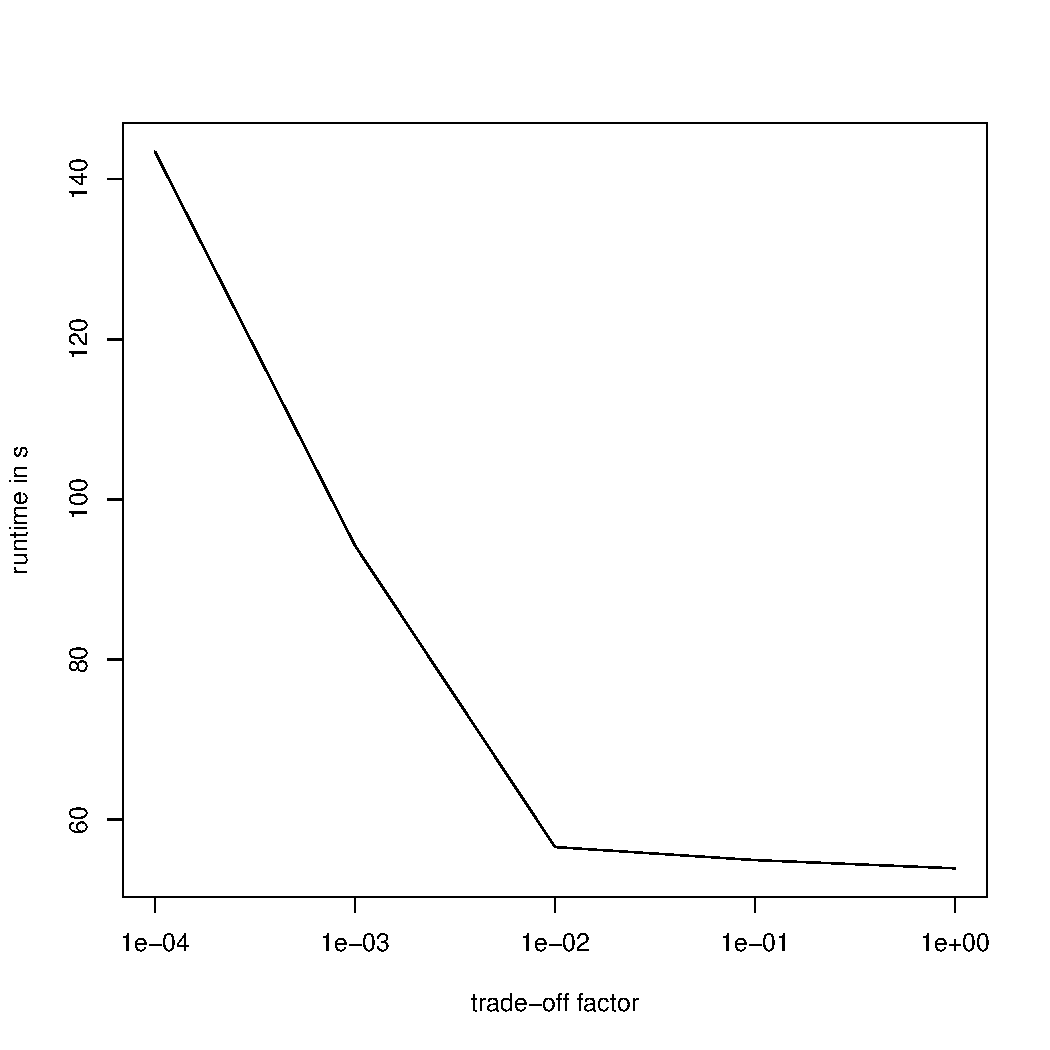
\includegraphics[width=0.45\textwidth]{../dia/runtime.pdf} }}
    	\caption{runtime and accuracy for given $lambda$}
    \end{figure}
\end{frame}

\begin{frame}[allowframebreaks]
	\frametitle{References}
	\nocite{*}
	\printbibliography
\end{frame}

\end{document}
